\documentclass{ximera}

%\usepackage{todonotes}

\newcommand{\todo}{}

\usepackage{esint} % for \oiint
\ifxake%%https://math.meta.stackexchange.com/questions/9973/how-do-you-render-a-closed-surface-double-integral
\renewcommand{\oiint}{{\large\bigcirc}\kern-1.56em\iint}
\fi


\graphicspath{
  {./}
  {ximeraTutorial/}
  {basicPhilosophy/}
  {functionsOfSeveralVariables/}
  {normalVectors/}
  {lagrangeMultipliers/}
  {vectorFields/}
  {greensTheorem/}
  {shapeOfThingsToCome/}
  {dotProducts/}
  {partialDerivativesAndTheGradientVector/}
  {../productAndQuotientRules/exercises/}
  {../normalVectors/exercisesParametricPlots/}
  {../continuityOfFunctionsOfSeveralVariables/exercises/}
  {../partialDerivativesAndTheGradientVector/exercises/}
  {../directionalDerivativeAndChainRule/exercises/}
  {../commonCoordinates/exercisesCylindricalCoordinates/}
  {../commonCoordinates/exercisesSphericalCoordinates/}
  {../greensTheorem/exercisesCurlAndLineIntegrals/}
  {../greensTheorem/exercisesDivergenceAndLineIntegrals/}
  {../shapeOfThingsToCome/exercisesDivergenceTheorem/}
  {../greensTheorem/}
  {../shapeOfThingsToCome/}
  {../separableDifferentialEquations/exercises/}
  {vectorFields/}
}

\newcommand{\mooculus}{\textsf{\textbf{MOOC}\textnormal{\textsf{ULUS}}}}

\usepackage{tkz-euclide}
\usepackage{tikz}
\usepackage{tikz-cd}
\usetikzlibrary{arrows}
\tikzset{>=stealth,commutative diagrams/.cd,
  arrow style=tikz,diagrams={>=stealth}} %% cool arrow head
\tikzset{shorten <>/.style={ shorten >=#1, shorten <=#1 } } %% allows shorter vectors

\usetikzlibrary{backgrounds} %% for boxes around graphs
\usetikzlibrary{shapes,positioning}  %% Clouds and stars
\usetikzlibrary{matrix} %% for matrix
\usepgfplotslibrary{polar} %% for polar plots
\usepgfplotslibrary{fillbetween} %% to shade area between curves in TikZ
%\usetkzobj{all}
\usepackage[makeroom]{cancel} %% for strike outs
%\usepackage{mathtools} %% for pretty underbrace % Breaks Ximera
%\usepackage{multicol}
\usepackage{pgffor} %% required for integral for loops



%% http://tex.stackexchange.com/questions/66490/drawing-a-tikz-arc-specifying-the-center
%% Draws beach ball
\tikzset{pics/carc/.style args={#1:#2:#3}{code={\draw[pic actions] (#1:#3) arc(#1:#2:#3);}}}



\usepackage{array}
\setlength{\extrarowheight}{+.1cm}
\newdimen\digitwidth
\settowidth\digitwidth{9}
\def\divrule#1#2{
\noalign{\moveright#1\digitwidth
\vbox{\hrule width#2\digitwidth}}}




% \newcommand{\RR}{\mathbb R}
% \newcommand{\R}{\mathbb R}
% \newcommand{\N}{\mathbb N}
% \newcommand{\Z}{\mathbb Z}

\newcommand{\sagemath}{\textsf{SageMath}}


%\renewcommand{\d}{\,d\!}
%\renewcommand{\d}{\mathop{}\!d}
%\newcommand{\dd}[2][]{\frac{\d #1}{\d #2}}
%\newcommand{\pp}[2][]{\frac{\partial #1}{\partial #2}}
% \renewcommand{\l}{\ell}
%\newcommand{\ddx}{\frac{d}{\d x}}

% \newcommand{\zeroOverZero}{\ensuremath{\boldsymbol{\tfrac{0}{0}}}}
%\newcommand{\inftyOverInfty}{\ensuremath{\boldsymbol{\tfrac{\infty}{\infty}}}}
%\newcommand{\zeroOverInfty}{\ensuremath{\boldsymbol{\tfrac{0}{\infty}}}}
%\newcommand{\zeroTimesInfty}{\ensuremath{\small\boldsymbol{0\cdot \infty}}}
%\newcommand{\inftyMinusInfty}{\ensuremath{\small\boldsymbol{\infty - \infty}}}
%\newcommand{\oneToInfty}{\ensuremath{\boldsymbol{1^\infty}}}
%\newcommand{\zeroToZero}{\ensuremath{\boldsymbol{0^0}}}
%\newcommand{\inftyToZero}{\ensuremath{\boldsymbol{\infty^0}}}



% \newcommand{\numOverZero}{\ensuremath{\boldsymbol{\tfrac{\#}{0}}}}
% \newcommand{\dfn}{\textbf}
% \newcommand{\unit}{\,\mathrm}
% \newcommand{\unit}{\mathop{}\!\mathrm}
% \newcommand{\eval}[1]{\bigg[ #1 \bigg]}
% \newcommand{\seq}[1]{\left( #1 \right)}
% \renewcommand{\epsilon}{\varepsilon}
% \renewcommand{\phi}{\varphi}


% \renewcommand{\iff}{\Leftrightarrow}

% \DeclareMathOperator{\arccot}{arccot}
% \DeclareMathOperator{\arcsec}{arcsec}
% \DeclareMathOperator{\arccsc}{arccsc}
% \DeclareMathOperator{\si}{Si}
% \DeclareMathOperator{\scal}{scal}
% \DeclareMathOperator{\sign}{sign}


%% \newcommand{\tightoverset}[2]{% for arrow vec
%%   \mathop{#2}\limits^{\vbox to -.5ex{\kern-0.75ex\hbox{$#1$}\vss}}}
% \newcommand{\arrowvec}[1]{{\overset{\rightharpoonup}{#1}}}
% \renewcommand{\vec}[1]{\arrowvec{\mathbf{#1}}}
% \renewcommand{\vec}[1]{{\overset{\boldsymbol{\rightharpoonup}}{\mathbf{#1}}}}

% \newcommand{\point}[1]{\left(#1\right)} %this allows \vector{ to be changed to \vector{ with a quick find and replace
% \newcommand{\pt}[1]{\mathbf{#1}} %this allows \vec{ to be changed to \vec{ with a quick find and replace
% \newcommand{\Lim}[2]{\lim_{\point{#1} \to \point{#2}}} %Bart, I changed this to point since I want to use it.  It runs through both of the exercise and exerciseE files in limits section, which is why it was in each document to start with.

% \DeclareMathOperator{\proj}{\mathbf{proj}}
% \newcommand{\veci}{{\boldsymbol{\hat{\imath}}}}
% \newcommand{\vecj}{{\boldsymbol{\hat{\jmath}}}}
% \newcommand{\veck}{{\boldsymbol{\hat{k}}}}
% \newcommand{\vecl}{\vec{\boldsymbol{\l}}}
% \newcommand{\uvec}[1]{\mathbf{\hat{#1}}}
% \newcommand{\utan}{\mathbf{\hat{t}}}
% \newcommand{\unormal}{\mathbf{\hat{n}}}
% \newcommand{\ubinormal}{\mathbf{\hat{b}}}

% \newcommand{\dotp}{\bullet}
% \newcommand{\cross}{\boldsymbol\times}
% \newcommand{\grad}{\boldsymbol\nabla}
% \newcommand{\divergence}{\grad\dotp}
% \newcommand{\curl}{\grad\cross}
%\DeclareMathOperator{\divergence}{divergence}
%\DeclareMathOperator{\curl}[1]{\grad\cross #1}
% \newcommand{\lto}{\mathop{\longrightarrow\,}\limits}

% \renewcommand{\bar}{\overline}

\colorlet{textColor}{black}
\colorlet{background}{white}
\colorlet{penColor}{blue!50!black} % Color of a curve in a plot
\colorlet{penColor2}{red!50!black}% Color of a curve in a plot
\colorlet{penColor3}{red!50!blue} % Color of a curve in a plot
\colorlet{penColor4}{green!50!black} % Color of a curve in a plot
\colorlet{penColor5}{orange!80!black} % Color of a curve in a plot
\colorlet{penColor6}{yellow!70!black} % Color of a curve in a plot
\colorlet{fill1}{penColor!20} % Color of fill in a plot
\colorlet{fill2}{penColor2!20} % Color of fill in a plot
\colorlet{fillp}{fill1} % Color of positive area
\colorlet{filln}{penColor2!20} % Color of negative area
\colorlet{fill3}{penColor3!20} % Fill
\colorlet{fill4}{penColor4!20} % Fill
\colorlet{fill5}{penColor5!20} % Fill
\colorlet{gridColor}{gray!50} % Color of grid in a plot

\newcommand{\surfaceColor}{violet}
\newcommand{\surfaceColorTwo}{redyellow}
\newcommand{\sliceColor}{greenyellow}




\pgfmathdeclarefunction{gauss}{2}{% gives gaussian
  \pgfmathparse{1/(#2*sqrt(2*pi))*exp(-((x-#1)^2)/(2*#2^2))}%
}


%%%%%%%%%%%%%
%% Vectors
%%%%%%%%%%%%%

%% Simple horiz vectors
\renewcommand{\vector}[1]{\left\langle #1\right\rangle}


%% %% Complex Horiz Vectors with angle brackets
%% \makeatletter
%% \renewcommand{\vector}[2][ , ]{\left\langle%
%%   \def\nextitem{\def\nextitem{#1}}%
%%   \@for \el:=#2\do{\nextitem\el}\right\rangle%
%% }
%% \makeatother

%% %% Vertical Vectors
%% \def\vector#1{\begin{bmatrix}\vecListA#1,,\end{bmatrix}}
%% \def\vecListA#1,{\if,#1,\else #1\cr \expandafter \vecListA \fi}

%%%%%%%%%%%%%
%% End of vectors
%%%%%%%%%%%%%

%\newcommand{\fullwidth}{}
%\newcommand{\normalwidth}{}



%% makes a snazzy t-chart for evaluating functions
%\newenvironment{tchart}{\rowcolors{2}{}{background!90!textColor}\array}{\endarray}

%%This is to help with formatting on future title pages.
\newenvironment{sectionOutcomes}{}{}



%% Flowchart stuff
%\tikzstyle{startstop} = [rectangle, rounded corners, minimum width=3cm, minimum height=1cm,text centered, draw=black]
%\tikzstyle{question} = [rectangle, minimum width=3cm, minimum height=1cm, text centered, draw=black]
%\tikzstyle{decision} = [trapezium, trapezium left angle=70, trapezium right angle=110, minimum width=3cm, minimum height=1cm, text centered, draw=black]
%\tikzstyle{question} = [rectangle, rounded corners, minimum width=3cm, minimum height=1cm,text centered, draw=black]
%\tikzstyle{process} = [rectangle, minimum width=3cm, minimum height=1cm, text centered, draw=black]
%\tikzstyle{decision} = [trapezium, trapezium left angle=70, trapezium right angle=110, minimum width=3cm, minimum height=1cm, text centered, draw=black]


\title{Euler's Formula}

\begin{document}

\begin{abstract}
complex exponentials
\end{abstract}
\maketitle






\subsection*{An Adventure}




One of the biggest surprises in mathematics is the fact that trigonometric functions and exponential functions are the same building blocks, provided we use Complex numbers. \\


Euler's Formula is the bridge:



\[    e^{i \, t} = \cos(t) + i \sin(t)    \]



This is very weird.  It claims that exponential functions are trigonometric functions are two perspectives on the same thing.  Our previous mathematcis courses have never even hinted at such a connection.  That is because the bridge  travels through the Complex Numbers.



With this bridge, we now have direct connections between


\begin{itemize}
\item percentage growth
\item exponential functions
\item trigonometric functions
\item triangles
\item circles
\end{itemize}

This would also connect inverse trigonometric functions and logarithms and soon hyperbolas and hyperbolic trigonometric functions.  This is crazy!


\begin{center}
\textbf{\textcolor{red!80!black}{Everything is Connected!!!}}
\end{center}






It would be nice to show that Euler's Formula is true.  However, we will need Calculus to dot our i's and cross our t's and leave no doubt.   But, we can understand the basic idea. 


To see that Euler's Formula is true, we need several pieces of information. \\





We have already seen that the derivative of $\sin(x)$ is $\cos(x)$ and derivative of $\cos(x)$ is $-\sin(x)$.

We need one more derivative.



\subsection*{Derivatives} 


\textbf{\textcolor{purple!85!blue}{Step A)}}

$\blacktriangleright$ We would like the derivative of $f(x) = e^{r \, x}$. \\


$f'(a)$ would be the slope of the tangent line at the point $(a, e^{r \, a})$. \\










\begin{image}
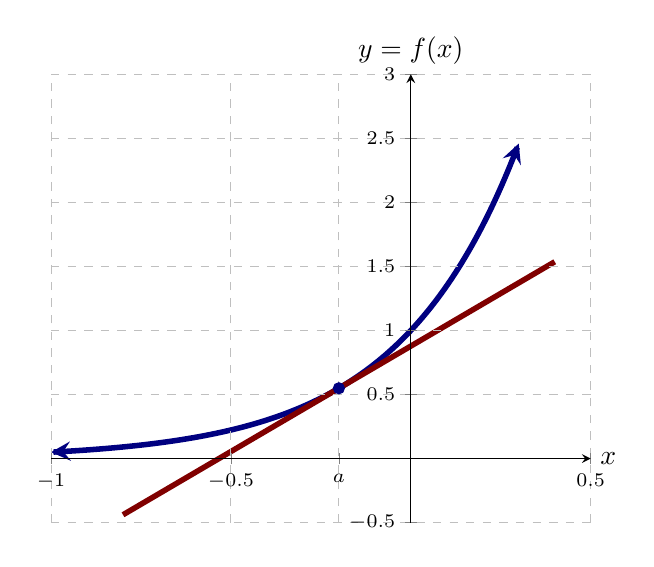
\begin{tikzpicture}
  \begin{axis}[
            domain=-1:0.5, ymax=3, xmax=0.5, ymin=-0.5, xmin=-1,
            axis lines =center, xlabel=$x$, ylabel={$y=f(x)$}, grid = major, grid style={dashed},
            ytick={-0.5,0,0.5,1,1.5,2,2.5,3},
            xtick={-1,-0.5,-0.2,0,0.5},
            yticklabels={$-0.5$,$0$,$0.5$,$1$,$1.5$,$2$,$2.5$,$3$}, 
            xticklabels={$-1$,$-0.5$,$a$,$0$,$0.5$},
            ticklabel style={font=\scriptsize},
            every axis y label/.style={at=(current axis.above origin),anchor=south},
            every axis x label/.style={at=(current axis.right of origin),anchor=west},
            axis on top
          ]
          
			\addplot [line width=2, penColor, smooth,samples=200,domain=(-1:0.3),<->] {2.718^(3*x)};


			\addplot[color=penColor,fill=penColor,only marks,mark=*] coordinates{(-0.2,0.5488)};
			\addplot [line width=2, penColor2, smooth,samples=200,domain=(-0.8:0.4)] {1.646*(x+0.2)+0.5488};


           

  \end{axis}
\end{tikzpicture}
\end{image}


That's what we want.  However, we don't know the derivative of $e^{r x}$, so we can't get the slope of the tangent line. \\

So, let's approximate the slope by using some close chords on the graph. \\



Let's pick two points on the graph of $e^{r x}$ and near $(a, e^{r a})$.  We'll pick
\[
(a-h, e^{r(a-h)}) \, \text{ and } \, (a+h, e^{r(a+h)})
\]

These two points are both on the graph and they are close to $(a, e^{r a})$ as long as $h$ is really small. \\

The slope of the line through these two point is 
\[
\frac{e^{r(a+h)} - e^{r(a-h)}}{2h}
\]




\begin{example}  $f(x) = e^{3 x}$

\begin{center}
\desmos{3ohrxje6e7}{400}{300}
\end{center}



Slide the value of $h$ closer to $0$.  Watch what happens to the secant line.

\end{example}





The slope of the secant line is really close to the slope of the tangent line. \\

The smaller the value of $h$, the closer the slopes are. \\


\[
\lim_{h \to 0} \frac{e^{r(a+h)} - e^{r(a-h)}}{2h} = \, \text{ slope of tangent at }a \, = f'(a)
\]


Move the tangent point along the curve by varying $a$.  Everytime you reposition $a$, you can slide the value of $h$ closer to $0$ and watch what happens with the sectant line.  It gets closer to the tangent line.  The slope of the secant line gets closer to the slope of the tangent line.

If we reposition $a$ a lot and we collect these slopes for a lot of $a$'s, then we could plot each of the slope values forming another graph.
\[   (a, f'(a)) \]



Let's do this for $r = 3$.

\begin{example}



Let's compare the plot of tangent slopes to the graph of $3 e^{3 x}$


The dashed curve is for $3 e^{3 x}$.

The plotted dot is $(a, f'(a))$.

\begin{example}  $f(x) = e^{3 x}$

\begin{center}
\desmos{5rjkc2evu0}{400}{300}
\end{center}

\end{example}





This is very suggestive that the derivative of $f(x) = e^{3 x}$ is $f'(x) = 3 e^{3 x}$.



\end{example}





It is not a far jump to believe that 




\begin{idea}

\[
\text{The derivative of } \, f(x) = e^{r x} \, \text{ is } \, f'(x) = r \, e^{r x}
\]


\[
\frac{d}{dx} e^{r x}  = r \, e^{r x}
\]

\end{idea}



That was \textbf{\textcolor{purple!85!blue}{Step A)}}. \\





\section*{Mean Value Theorem}

\textbf{\textcolor{purple!85!blue}{Step B)}} \\

In Calculus, you will study the \textbf{Mean Value Theorem}. One version follows this race track story:


Suppose two horses are racing.  They both line up at the starting line.  During the race, they both run at exactly the same speed at every second of the race.  Under these circumstances, the two horses are at exactly the same place on the track at every second of the race and end the race in a tie.




In function language, the story goes like this:

Suppose 

\begin{itemize}
\item $f$ and $g$ are two functions,
\item $f(0) = g(0)$, and
\item $f'(t) = g'(t)$  for all $t$.
\end{itemize}

Then $f(t)=g(t)$ for all $t$.   $f$ and $g$ are the same function.



If two functions start with the same value and then they have the exact same derivative everywhere, then they are the same function. \\









$\blacktriangleright$  When you study differential equations, this idea will lead to the fact that a first-order differential equation with an initial condition has only one solution. \\

\textbf{\textcolor{blue!55!black}{Example: }} If $y'(t) = k \cdot y(t)$ with $y(0)=1$


There is only one function that could be $y(t)$.  $y(t) = e^{k t}$

Let's apply this to our situation. \\















\section*{Euler's Formula}


\textbf{\textcolor{purple!85!blue}{Step C)}} \\


That Mean Value Theorem horse race story was for real numbers, but we are going to take a slight leap of faith and extend it to complex numbers.




Consider these two functions:


\begin{itemize}
	\item $f(t) = e^{i t}$
	\item $g(t) = \cos(t) + i \sin(t)$
\end{itemize}




$\blacktriangleright$   \textbf{Step 1:} Our functions have the same initial value.

\begin{itemize}
	\item $f(0) = e^0 = 1$
	\item $g(0) = \cos(0) + i \sin(0) = 1$
\end{itemize}





$\blacktriangleright$   \textbf{Step 2:} Our functions satisfy the same differential equation: $y'(t) = i \cdot y(t)$



\begin{itemize}
	\item $f'(t) = i \, e^{i \, t} = i \, f(t)$
	\item $g'(t) = -\sin(t) + i \cos(t) = i \, g(t)$
\end{itemize}



We have two functions satisfying the same differential equation with the same initial value.  They must, in fact, be the same function. \\




\begin{theorem} \textbf{\textcolor{green!50!black}{Euler's Formula}}   


\[   e^{i \, t} = \cos(t) + i \sin(t)         \]



$t$ is called the \textbf{argument}, often shortened to \textbf{\textcolor{green!50!black}{$arg$}}.  

\end{theorem}




Euler's Formula is a bridge between exponential functions and trigonometric functions. \\


\begin{center}

It is pronounced ``\textit{Oiler}''.


\end{center}


Complex Numbers are described by polar coordinates, which are connected to right triangles, which are similar to right triangles on the unit circle, which are built from sine and cosine, which are now connected to complex exponentials.




\begin{center}


\[
a + b \, i =  r \cdot (\cos(\theta) + i \, \sin(\theta)) = r \cdot e^{i \cdot \theta}
\]

\end{center}


Complex numbers can be written in exponential form, just like real numbers can.  They just need complex exponents.



\begin{example}


Let $z = \frac{5}{2} + \frac{5\sqrt{3}}{2} \, i$

The modulus of $z$ is $\answer{5}$ 

$arg(z) = \answer{\frac{\pi}{3}}$


$z = \frac{5}{2} + \frac{5\sqrt{3}}{2} \, i = 5 \, e^{i \tfrac{\pi}{3}}$

\end{example}




Of course, we can also write $5$ as $e^{\ln(5)}$.


$z = \frac{5}{2} + \frac{5\sqrt{3}}{2} \, i = 5 \, e^{i \tfrac{\pi}{3}} = e^{\ln(5)} \, e^{i \tfrac{\pi}{3}} = e^{\ln(5) + i \tfrac{\pi}{3}}$












\begin{center}
\textbf{\textcolor{green!50!black}{ooooo-=-=-=-ooOoo-=-=-=-ooooo}} \\

more examples can be found by following this link\\ \link[More Examples of Complex Bridge]{https://ximera.osu.edu/csccmathematics/precalculus2/precalculus2/complexBridge/examples/exampleList}

\end{center}







\end{document}
